
%-=-=-=-=-=-=-=-=-=-=-=-=-=-=-=-=-=-=-=-=-=-=-=-=
%
%        LOADING DOCUMENT
%
%-=-=-=-=-=-=-=-=-=-=-=-=-=-=-=-=-=-=-=-=-=-=-=-=

%jkuColors: white, black, jkuGrey, jkuBlue, jkuCyan, jkuGreen, jkuLightGreen, jkuYellow, jkuPurple, jkuRed 
\documentclass[9pt, english]{beamer}

\setbeamertemplate{caption}[numbered]

% -=-=-=-=-=-=-=-=-=-=-=-=-=-=-=-=-=-=-=-=-=-=-=-=-=-=-=-=-=-=
% Choose among the following options for the JKU-beamer-theme:
% -=-=-=-=-=-=-=-=-=-=-=-=-=-=-=-=-=-=-=-=-=-=-=-=-=-=-=-=-=-=
% german
% protectframetitle
% nopagenumber
% nosectionpage
% nojkuFooter
% greyText
% RE
% SOWI
% TNF
% MED
% mac
\usetheme[TNF]{jku}
\setbeamerfont{frametitle}{size=\huge}

%-=-=-=-=-=-=-=-=-=-=-=-=-=-=-=-=-=-=-=-=-=-=-=-=
%        LOADING PACKAGES
%-=-=-=-=-=-=-=-=-=-=-=-=-=-=-=-=-=-=-=-=-=-=-=-=
\usepackage[utf8]{inputenc}
\usepackage[font={footnotesize, it}]{caption}

\usepackage{hyperref}
\usepackage[normalem]{ulem}

% \usepackage{caption}
% \usepackage{subcaption}

\usepackage{amsmath}
\usepackage{amssymb}
\usepackage{mathtools}
\usepackage{physics}

\newcommand{\pvec}[1]{\vec{#1}\mkern2mu\vphantom{#1}}
\renewcommand{\d}{\mathrm{d}}
\newcommand{\CPP}{C\texttt{++} }

\graphicspath{ {images/} }

%-=-=-=-=-=-=-=-=-=-=-=-=-=-=-=-=-=-=-=-=-=-=-=-=
%
%	PRESENTATION INFORMATION
%
%-=-=-=-=-=-=-=-=-=-=-=-=-=-=-=-=-=-=-=-=-=-=-=-=

\title{Recurrence Quantitative Analysis of Particulate Systems}
\subtitle{Short Talk}
\author{Thomas Miethlinger B.Sc.}
% \institute{Department of Particulate Flow Modelling}
\date{19.12.2019}
\partnerlogo{hzdr_logo.png}

\bibliographystyle{abbrv}

\begin{document}

% \jkulogogrey

\jkulogowhite

%-=-=-=-=-=-=-=-=-=-=-=-=-=-=-=-=-=-=-=-=-=-=-=-=
%
%	TITLE PAGE
%
%-=-=-=-=-=-=-=-=-=-=-=-=-=-=-=-=-=-=-=-=-=-=-=-=

\maketitle

\section{Preliminary}

%-=-=-=-=-=-=-=-=-=-=-=-=-=-=-=-=-=-=-=-=-=-=-=-=
%
%	Frame: About Me
%
%-=-=-=-=-=-=-=-=-=-=-=-=-=-=-=-=-=-=-=-=-=-=-=-=

\begin{frame}
\frametitle{Acknowledgment}
I want to sincerely thank:
\begin{itemize}
 \item Dr. Thomas Kluge for the invitation and organization of my stay
 \item The Institute of Radiation Physics for their time, the possibility to get to know their research facilities and the financial support for my travel
\end{itemize}
\end{frame}

%-=-=-=-=-=-=-=-=-=-=-=-=-=-=-=-=-=-=-=-=-=-=-=-=
%
%	Frame: About Me
%
%-=-=-=-=-=-=-=-=-=-=-=-=-=-=-=-=-=-=-=-=-=-=-=-=

\begin{frame}
\frametitle{About Me}
\begin{columns}[t]
\begin{column}{0.65\textwidth}
\vspace{-0.25cm}
\begin{itemize}
 \item Master Student at Johannes Kepler University Linz
 \item Study: Technical Physics
 \item Selection of courses / topics:
  \begin{itemize}
  \item Computational Physics 
  \begin{itemize}
   \item Quantum: Density Functional Theory, Quantum Monte Carlo
   \item Classical: Molecular Dynamics, Monte Carlo
   \item Computational Fluid Dynamics
  \end{itemize}
  \item Quantum Many-Body Theory, Quantum Chemistry, Quantum Solid State Physics
  \item Fluid Dynamics Theory
  \item Laser Physics, Photonics
  \item High Performance Computing
  \begin{itemize}
   \item Experience: OpenMP, MPI, HPX
   \item Little experience, but interested in: CUDA, GPGPU programming
  \end{itemize}
 \end{itemize}
\end{itemize}
\end{column}
\begin{column}{0.35\textwidth}
\begin{figure}
\centering
\includegraphics[width=1.0\textwidth]{route_jku_hzdr.png}
\end{figure}
\end{column}
\end{columns}
\end{frame}

%-=-=-=-=-=-=-=-=-=-=-=-=-=-=-=-=-=-=-=-=-=-=-=-=
%
%	SECTION: INTRODUCTION 
%
%-=-=-=-=-=-=-=-=-=-=-=-=-=-=-=-=-=-=-=-=-=-=-=-=

\section{Recurrence Quantitative Analysis of Particulate Systems}

\begin{frame}
\frametitle{Motivation}
\begin{itemize}
 \item Long-time simulations with a fairly high degree of accuracy are computationally expensive
 \begin{itemize}
 \item In this work: CFDEM\footnote{Computational Fluid Dynamics + Discrete Element Method} simulation of a technical process
 \item Current trend: Data-assisted calculations/simulations(``hybrid-models'')
 \end{itemize}
 \item Conceptual questions 
 \item Curiosity
\end{itemize}
\end{frame}

\begin{frame}
\frametitle{Recurrence Quantitative Analysis}
\begin{itemize}
 \item Abbreviated as RQA
 \item Set of techniques and methods for the investigation of dynamical systems
 \item Based on Non-Linear Dynamical Systems and Chaos Theory
 \item Central quantities:
 \begin{itemize}
  \item State of the system: \(x\)
  \item Distance (between state \(A\) and state \(B\)) function: \(d(x_A,x_B) = \lvert \lvert x_A - x_B \rvert \rvert\)
  \item Recurrence function: \(R_{\epsilon}(x_A,x_B) = \Theta(\epsilon - d_{\mathcal{N}}(x_A,x_B))\); visualized as recurrence plot (RP).
  %   \item Distance (between state \(A\) and state \(B\)) function: \(d(\vb{x}_A,\vb{x}_B) = \lvert \lvert \vb{x}_A - \vb{x}_B \rvert \rvert\)
%   \item Recurrence function: \(R_{\epsilon}(\vb{x}_A,\vb{x}_B) = \Theta(\epsilon - d(\vb{x}_A,\vb{x}_B))\)
 \end{itemize}
 \item Many derived quantities:
 \begin{itemize}
  \item Recurrence Rate \(RR_{\epsilon}\)
  \item Determinism DET \(DET_{\epsilon}\)
  \item Trapping Time \(TT_{\epsilon}\)
  \item Correlation Dimension \(\nu\)
  \item Lyapunov Exponents \(\{\lambda_k\}\)
 \end{itemize}
\end{itemize}
\end{frame}

\begin{frame}[fragile]
\frametitle{Example Recurrence Plot}
\begin{figure}
\centering
\includegraphics[width=0.625\textwidth]{recurrence_plot_example.png}
\caption{Example of a recurrence plot with \(\epsilon=0.2\).}
\end{figure}
\end{frame}

\begin{frame}
\frametitle{Distance Function: General}
Required for RQA: Measure of distance between two arbitrary states.
Typical distance functions for finite-dimensional state vectors\footnote{Infinite-dimensions: \(\sum \rightarrow \int\)}:
\begin{enumerate}
 \item Manhattan distance (\(L^1\) distance): \(d_1(x_A,x_B) = \lvert \lvert x_A - x_B \rvert \rvert_1 = \sum_i{\lvert x_{A,i} - x_{B,i}\rvert}\)
 \item Euclidean distance (\(L^2\) distance): \(d_2(x_A,x_B) = \lvert \lvert x_A - x_B \rvert \rvert_2 = \sqrt{\sum_i{(x_{A,i} - x_{B,i})^2}}\)
\end{enumerate}
\end{frame}

\begin{frame}
\frametitle{Distance Function for Classical Particles}
Assumptions:
\begin{itemize}
 \item Identical particles
 \item Number of particles \(N\)
 \item Point particles\footnote{for simplicity in this talk} \(\rightarrow\) mass density distribution \( = \delta(\lvert \vb{r} - \vb{r}_{\text{particle}} \rvert)\)
%  \item Spherical particles with mass density distribution \(G(\lvert \vb{r} - \vb{r}_{\text{particle}} \rvert)\)
\end{itemize}
Two mathematically different descriptions to define state of system:
\begin{enumerate}
 \item Momentum density field
 \item Phase space vector
\end{enumerate}
\end{frame}

\begin{frame}
\frametitle{Distance Function for Classical Particles}
\begin{columns}[t]
\begin{column}{0.45\textwidth}
\vspace{0.25cm}
Momentum density field:
\[
 x = \sum_{i=1}^N{\vb{p}_i \delta(\vb{r} - \vb{r}_i)}
\]
\vspace{0.2cm}
\begin{itemize}
 \item Infinite-dimensional (Function space)
 \item Invariant to particle permutation
\end{itemize}
\vspace{0.2cm}
\[
 d(x_A,x_B)
        \begin{cases}
         = 0\text{, if } x_A = x_B \\
         \rightarrow \infty\text{, if } x_A \neq x_B 
        \end{cases}
\]
\(\rightarrow\) Adaption needed for finite distance
\end{column}
\begin{column}{0.49\textwidth}
Phase space vector:
\vspace{0.1cm}
\[
        x = 
        \big(\vb{R} \; \vb{P}\big) = 
        \left(
        \begin{array}{c}
         ... \\
         \vb{r}_i \; \vb{p}_i \\
%         x_i \, y_i \, z_i \, v_{x,i} \, v_{y,i} \, v_{z,i} \\
         ... \\
         \end{array}
        \right)
        \in \mathbb{R}^{6N}
\]
\begin{itemize}
 \item Finite-dimensional
 \item Not invariant to particle permutation
\end{itemize}
\vspace{0.95cm}
\[
 d(x_A,x_B) \in [0, \infty)
\]
\(\rightarrow\) Optimization w.r.t. particle permutations needed
\end{column}
\end{columns}
\end{frame}

% \begin{frame}
% \frametitle{Distance Function: Fields}
% Most intuitive way to compute the distance function of two different 
% Simplest way: \(L^2\) distance of convolved fields w.r.t. a convolution kernel\footnote{E.g. 3d box-kernel function or unit-sphere function} \(G\):
% Macroscopic momentum density field:
% \begin{equation}
%  \bar{\vb{p}}(\vb{r}) = (\vb{p} * G)(\vb{r}) = \sum_{i=1}^N{\vb{p}_i G(\lvert \vb{r} - \vb{r}_i \rvert)}
% \end{equation}
% \begin{equation}
%  d_{\text{Euler},p}(x_A,x_B) = \int_V{\lvert \bar{\vb{p}}_A(\vb{r}) - \bar{\vb{p}}_B(\vb{r}) \rvert^p \d^3 r}
% \end{equation}
% Problems:
% \begin{enumerate}
%  \item Shape and width \(\ell\) of \(G\) is arbitrary, but important:
%  \item Large \(\ell\) does not resolve small-scale information of the fields and induces higher-order effects
%  \item Small \(\ell\) does not take into account long displacements
% \end{enumerate}
% \end{frame}

\begin{frame}
\frametitle{Distance Functions: Positions and Number Densities}
For a better understanding of the relationship between those two distance functions,
in the beginning we only considered the positions \(\{\vb{r}_i\}\) and number density field 
\begin{equation}
 n(\vb{r}) = \sum_{i=1}^N{\delta(\lvert \vb{r} - \vb{r}_i \rvert)},
\end{equation}
i.e. we neglected momenta\footnote{\(\vb{p}_i \rightarrow 1\)}.
Most intuitive way to compute a finite distance between two different ``point clouds'' is by
computing the ``Eulerian''\footnote{\(L^2\) distance defined for function space} distance
\begin{equation}
 d_{\text{Euler}}(x_A,x_B) = \bigg( \int_V{(\bar{n}_A(\vb{r})-\bar{n}_B(\vb{r}))^2 \: \d^3 r} \bigg)^{1/2}
\end{equation}
of the mean number density field \(\bar{n}(\vb{r})\), which is defined w.r.t. a normalized convolution kernel \(G(r)\) by 
\begin{equation}
 \bar{n}(\vb{r}) = (n * G)(\vb{r}) = \sum_{i=1}^N{G(\lvert \vb{r} - \vb{r}_i \rvert)}.
\end{equation}
\end{frame}

\begin{frame}[fragile]
\frametitle{Importance of the Kernel \(G\)}
Problems with the Eulerian distance:
\begin{enumerate}
 \item Shape and size(defined by the kernel radius \(R\)) of \(G\) is arbitrary, but significant
 \item Large \(R \rightarrow\) does not resolve small-scale information of the fields and induces higher-order effects
 \begin{itemize}
  \item For \(R \propto L\) (system size): \(d_{\text{Euler}} \rightarrow 0\)
 \end{itemize}
 \item Small \(R \rightarrow\) does not take into account long displacements,
       since the Eulerian distance increases only as long as separation distance \(\delta r\) between two particles with radius \(R\) fulfills:
\end{enumerate}
\begin{equation}
 \delta r < 2 \cdot R.
\end{equation}
Otherwise, the overlap is and stays zero, since
\begin{equation}
 \int_V{\big(\bar{n}_A-\bar{n}_B\big)^2 \d^3 r} = \int_V{\big(\bar{n}_A^2-\underbrace{2\bar{n}_A\bar{n}_B}_{= 0 \text{ if } \delta r \geq 2 \cdot R}+\bar{n}_B^2\big) \: \d^3 r}.
\end{equation}
\end{frame}

\begin{frame}[fragile]
\frametitle{Eulerian Distance}
\begin{figure}
\centering
\includegraphics[width=.85\textwidth]{box_filter_distance.png}
\caption{Eulerian distance in dependence of separation distance of
the normalized box distribution (\(1\)d),
a normalized circular distribution (\(2\)d) and
a normalized spherical distribution (\(3\)d).}
\end{figure}
\end{frame}

\begin{frame}
\frametitle{Lagrangian Distance}
Eulerian distance has problems \(\rightarrow\) alternative is ``Lagrangian'' distance,
which is proposed\footnote{Bednarek et al. (2019): Extrapolation of DEM simulations to large time scale. Application to the mixing of powder in a conical screw mixer}\footnote{Zuk et al. (2018): Sampling rare events in stochastic reaction-diffusion systems within trajectory looping} as follows:
\begin{equation}
 d_{\text{Lagrangian}}(x_A,x_B) = \sum_{i=1}^N{\lvert \vb{r}_{A,i} - \vb{r}_{B,j_i} \rvert} =: \sum_{i=1}^N{\delta r_i}
\end{equation}
I.e. we to calculate the \textit{\textbf{global}} separation between state \(A\) and state \(B\) by summing up the \sout{\textit{\textbf{local}}} \textit{\textbf{discrete}} separation distances.:
\begin{enumerate}
 \item We must find an \textit{unique matching} \(j_i\) from state \(B\) for each particle \(i\) from state \(A\)
 \item Combinatorial problem: \(N!\) matching possibilities
 \item Only interested in the best matching, i.e. the pairs \((i,j_i)\) such that
 \begin{equation}
  \sum_{i=1}^N{\delta r_i} \stackrel{\text{!}}{=} \min_{\{j_i\}}{}.
 \end{equation}
\end{enumerate}
\vspace{+0.3cm}
\end{frame}

\begin{frame}
\frametitle{Hungarian Algorithm}
The Hungarian Algorithm computes the solve the assignment problem in polynomial time.
There are two different approaches:
\begin{enumerate}
 \item Slow approaches with \(\mathcal{O}(N^4)\) or \(\mathcal{O}(N^5)\).
 Derived by matrix operations, and not so difficult to understand.
 \item Fast approach with \(\mathcal{O}(N^3)\).
 Derived by graph operations\footnote{A nice introduction to the Hungarian Algorithm is given e.g. \url{https://www.topcoder.com/community/competitive-programming/tutorials/assignment-problem-and-hungarian-algorithm/}}, and is more involved to understand.
\end{enumerate}
\begin{center}
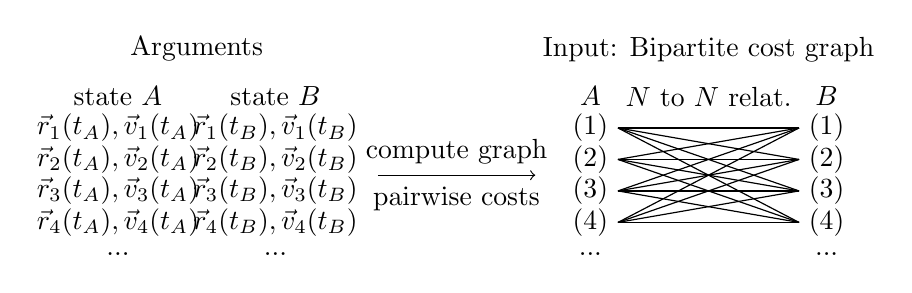
\begin{tikzpicture}[
x=1cm,
y=1cm,
tasknode/.style={rectangle, draw=blue!60, fill=blue!5, very thick, minimum height=1cm},
]
\node at (-2cm,0.6cm) {Arguments};
\node at (-3cm,0.0) {\(\text{state }A\)};
\node at (-1cm,0.0) {\(\text{state }B\)};
\node at (4.5cm,0.6cm) {Input: Bipartite cost graph};
\foreach \i in {1,...,4}
{
 \node at (-3cm,-\i*0.4) {\(\vec{r}_{\text{\i}}(t_A),\vec{v}_{\text{\i}}(t_A)\)};
 \node at (-1cm,-\i*0.4) {\(\vec{r}_{\text{\i}}(t_B),\vec{v}_{\text{\i}}(t_B)\)};
}
\node at (-3cm,-2) {...};
\node at (-1cm,-2) {...};
\node at (1.3,-1+0.3) {compute graph};
\node at (1.3,-1-0.3) {pairwise costs};
\draw[->,line width=0.15mm] (0.3,-1) -- (2.3,-1);
\node[rectangle] at (3cm,0.0) {\(A\)};
\node[rectangle] at (4.5cm,0.0) {\(N\) to \(N\) relat.};
\node[rectangle] at (6cm,0.0) {\(B\)};
\foreach \i in {1,...,4}
{
\node[rectangle] at (3cm,-\i*0.4) {\((\text{\i})\)};
\node[rectangle] at (6cm,-\i*0.4) {\((\text{\i})\)};
 \foreach \j in {1,...,4}
 {
  \draw[-,line width=0.15mm] (3cm+0.35cm,-\i*0.4) -- (6cm-0.35cm,-\j*0.4);
 }
}
\node at (3cm,-2) {...};
\node at (6cm,-2) {...};
\end{tikzpicture}
\end{center}
\end{frame}

\begin{frame}
\frametitle{Literature search: Hungarian Algorithm}
\begin{enumerate}
 \item Numerous implementations with \(\mathcal{O}(N^4)\) and \(\mathcal{O}(N^5)\).
 \item DLIB\footnote{King (2009). Dlib-ml: A machine learning toolkit. \url{dlib.net}}. General \CPP library, \(\mathcal{O}(N^3)\).
 \item t3nsor/codebook\footnote{\url{https://github.com/t3nsor/codebook}, ``Unlicensed'' license}. Support material for ACM-ICPC World Finals, \(\mathcal{O}(N^3)\).
 \item sKM algorithm\footnote{Cui, Zhang et al. (2016): Solving large-scale assignment problems by Kuhn-Munkres algorithm}, \(\mathcal{O}(N^2N_{\text{egde}})\) implementation. Tried contact, but no response.\item DHA\footnote{Ayorkor et al. (2007): The Dynamic Hungarian Algorithm for the Assignment Problem with Changing Costs}. Potentially very useful. Tried contact, but no response
\end{enumerate}
\end{frame}

\begin{frame}
\frametitle{Hungarian Algorithm for Sparse Cost Matrix}
\begin{itemize}
 \item Conventional Hungarian Algorithm uses \textit{\textbf{bipartite graph}} (\(N\) to \(N\) relationship), which is represented by a \textit{cost adjacency matrix}. As already stated, it can be solved in \(\mathcal{O}(N^3)\).
 \item Sparse Hungarian Algorithm uses a \textit{\textbf{non-bipartite graph}} (\(N\) to \(N_{\text{edge}}\) relationship), which is represented by \textit{cost adjacency lists}. Based on literature search\footnote{Cui, Zhang et al. (2016): Solving large-scale assignment problems by Kuhn-Munkres algorithm}, such a algorithm is possible to implement.
 \end{itemize}
First major task: program HA based on cost adjacency lists, which (hopefully) runs in \(\mathcal{O}(N^2 N_{\text{edge}})\).
\newline
Results: First only \(\mathcal{O}(N^2 N_{\text{edge}} \log{(N_{\text{edge}})})\), but current version is \(\mathcal{O}(N^2 N_{\text{edge}})\).
\end{frame}

\section{Results}

\begin{frame}[fragile]
\frametitle{Sparse Hungarian Algorithm: Absolute Run Times}
\begin{figure}
\centering
\includegraphics[width=.85\textwidth]{ha_t3nsor_runtimes_absolute.png}
\caption{Absolute run times of the original \(t_{\text{t3nsor}}(N)\) in comparison to the adapted \(t_{\text{t3nsor}}(N,N_{\text{edge}})\) based on adjacency lists. One can see a strong benefit by using \(N_{\text{edge}} < N\) edges.}
\end{figure}
\end{frame}

\begin{frame}[fragile]
\frametitle{Sparse Hungarian Algorithm: Efficiency}
\begin{figure}
\centering
\includegraphics[width=.85\textwidth]{ha_t3nsor_runtimes_efficiency.png}
\caption{Run time efficiency of the adapted \(t_{\text{t3nsor}}(N,N_{\text{edge}})\) based on adjacency lists. The average efficiency appears to be around \(0.7\), i.e. \(30\%\) slower than the theoretical limit.}
\end{figure}
\end{frame}

\begin{frame}[fragile]
\frametitle{System: Fluidized Bed}
\begin{figure}
\centering
\includegraphics[width=0.825\textwidth]{fludidized_bed_evolution_5_2_low.jpg}
\caption{Snapshots of the system, which is a fluidized bed with \(N=50000\) particles.}
\end{figure}
\end{frame}

\begin{frame}[fragile]
\frametitle{Qualitative Comparison}
\begin{columns}[t]
\begin{column}{0.5\textwidth}
\vspace{-0.65cm}
\begin{figure}
\centering
\includegraphics[width=0.7\textwidth]{fludidized_bed_displacement_1.png}
\caption{Displacement field for two states of medium degree of difference.}
\end{figure}
\end{column}
\begin{column}{0.5\textwidth}
\vspace{-0.65cm}
\begin{figure}
\centering
\includegraphics[width=0.7\textwidth]{fludidized_bed_displacement_2.png}
\caption{Displacement field for two states of high degree of difference.}
\end{figure}
\end{column}
\end{columns}
\end{frame}

\begin{frame}[fragile]
\frametitle{Qualitative Comparison}
\begin{columns}[t]
\begin{column}{0.56\textwidth}
\begin{figure}
\centering
\includegraphics[width=1\textwidth]{field_distance_matrix_5_30_8_8_8.jpg}
\caption{Normalized distance matrix w.r.t. Eulerian distance (kernel: large \(R\)).}
\end{figure}
\end{column}
\begin{column}{0.56\textwidth}
\begin{figure}
\centering
\includegraphics[width=1\textwidth]{discrete_distance_matrix_5_30_6000_6000.jpg}
\caption{Normalized distance matrix w.r.t. Lagrangian distance.}
\end{figure}
\end{column}
\end{columns}
\end{frame}

\begin{frame}[fragile]
\frametitle{Qualitative Comparison}
\begin{columns}[t]
\begin{column}{0.56\textwidth}
\begin{figure}
\centering
\includegraphics[width=1\textwidth]{field_distance_matrix_5_30_12_12_12.jpg}
\caption{Normalized distance matrix w.r.t. Eulerian distance (kernel: small \(R\)).}
\end{figure}
\end{column}
\begin{column}{0.56\textwidth}
\begin{figure}
\centering
\includegraphics[width=1\textwidth]{discrete_distance_matrix_5_30_6000_6000.jpg}
\caption{Normalized distance matrix w.r.t. Lagrangian distance.}
\end{figure}
\end{column}
\end{columns}
\end{frame}

\section{Conclusion and Outlook}

\begin{frame}[fragile]
\frametitle{Conclusion and Outlook}
\begin{itemize}
 \item Performed long-time simulation of technical process(fluidized bed).
 \item Implemented sHA with \(\approx 70\%\) efficiency\footnote{Currently in private repo: \url{https://github.com/ThomasMiethlinger/master_thesis_work/tree/master/programs/src/hungarian_algorithm}}
 \item Theoretical work: \(d_{\text{Euler}} \stackrel{\text{?}}{\leftrightarrow} d_{\text{Lagrange}}\), implications for RQA quantities
 \begin{itemize}
  \item Results show: Leading order depends on kernel shape, coefficient on kernel size / radius \(R\).
  \item Most quantities depend strongly on distance function, correlation dimension appears invariant to choice \(d_{\text{Euler}}\), \(d_{\text{Lagrange}}\)
 \end{itemize}
 \item Computational work:
 \begin{itemize}
  \item compute distance / recurrence matrices for \(d_{\text{Euler}}, d_{\text{Lagrange}}\) with different kernels and powers
  \item RQA of computed recurrence matrices
 \end{itemize}
\end{itemize}
\end{frame}

\jkulogowhite

% \begin{frame}
% \frametitle{Distance Functions: Positions only}
% Assuming the particles of the two different states have similar positions \(\{\vb{r}_i\}\) and \(\{\vb{r}_i'=\vb{r}_i+\delta\vb{r}_i\}\),
% the local difference of the mean number density field
% \begin{equation}
%  \delta\bar{n}(\vb{r}) = \sum_{i=1}^N{G(\lvert \vb{r} - (\vb{r}_i + \delta\vb{r}_i) \rvert) - G(\lvert \vb{r} - \vb{r}_i \rvert)}
% \end{equation}
% can be approximated for a smooth kernel in first order with
% \begin{equation}
%  \delta\bar{n}(\vb{r}) \approx \sum_{i=1}^N{\delta\vb{r}_i \cdot \nabla G(\lvert \vb{r} - \vb{r}_i \rvert)}.
% \end{equation}
% For similar configurations and sufficiently short-ranged\footnote{Such that \(\nabla G(\lvert \vb{r} - \vb{r}_i \rvert)\nabla G(\lvert \vb{r} - \vb{r}_j \rvert) \rightarrow 0 \text{ if } i \neq j \)} \(G(r)\), we find
% \begin{equation}
%  \int_V{ \delta\bar{n}(\vb{r})^2 \: \d^3 r} \propto \sum_{i=1}^N{\delta\vb{r}_i^2}.
% \end{equation}
% \end{frame}
% 
% \begin{frame}
% \frametitle{Distance Functions: Positions only}
% However, our data shows
% \end{frame}


% \begin{equation}
%  d_{\text{Euler},p}(x_A,x_B) = \int_V{\lvert \bar{n}_A(\vb{r}) - \bar{n}_B(\vb{r}) \rvert^p \d^3 r}
% \end{equation}
% \begin{frame}
% \frametitle{Particle Permutations: Assignment Problem}
% Given two particulate systems \(A\) and \(B\) consisting both of \(N\) particles,
% match each particle from system \(A\) to a particle from system \(B\) uniquely such that the total distance is minimized:
% 
% 
% 
% 
% 
% 
% Given \(N\) particles at two different times \(t_a\) and \(t_b\),
% we want to calculate the \textit{\textbf{global}} seperation between both,
% by using the \sout{\textit{\textbf{local}}} \textit{\textbf{discrete}} seperation distances\footnote{and possibly also the velocity difference \(\Delta v\)}, for example by computing:
% \begin{equation}\label{objfunc}
%   D_{t_a,t_b}=\sum_{i=1}^N{ \lvert \vec{r}_i(t_a) - \vec{r}_{q_i}(t_b) \rvert}=\sum_{i=1}^N{\Delta r_{iq_i}(t_a,t_b)}.
% \end{equation}
% \begin{enumerate}
%  \item We must find an \textit{unique matching} \(q_i\) for each particle \(i\)
%  \item However, there are \(N!\) matching possibilities!
%  \item But we are only interested in the best matching, i.e. the pairs
%  \begin{equation}
%   \{ i \rightarrow q_i = j \}_{1\leq i \leq N},
%  \end{equation}
%  such that
%  \begin{equation}
%   \sum_{i=1}^N{\Delta r_{iq_i}} \stackrel{\text{!}}{=} \min_{\{q_i\}}{}.
%  \end{equation}
% \end{enumerate}
% 
% 
% 
% 
% 
% 
% 
% \end{frame}

% \begin{frame}
% \frametitle{Project Idea: Starting Points (cont.)}
% \begin{itemize}
%   \item Next step: recurrence quantitative analysis of particles
%  \begin{itemize}
%   \item Existing: theoretical frameworks for few \textit{distinguishable} particles\footnote{Dynamical Systems Theory, Chaos Theory and Perturbation Theory}. What about (few or many) \textit{identical} particles?
%   \item Existing: computational framework. (``Hungarian Algorithm'' or ``Kuhn-Munkres Algorithm'')
%    \begin{enumerate}
%     \item Numerous implementations with \(\mathcal{O}(N^4)\) and \(\mathcal{O}(N^5)\).
%     \item DLIB\footnote{King (2009). Dlib-ml: A machine learning toolkit. \url{dlib.net}}. General \CPP library. Has a \(\mathcal{O}(N^3)\) implementation.
%     \item t3nsor/codebook\footnote{\url{https://github.com/t3nsor/codebook}, ``Unlicenced'' license}. Support material for ACM-ICPC World Finals. Has a fast \(\mathcal{O}(N^3)\) implementation. 
%     \item sKM algorithm\footnote{Cui, Zhang et al. (2016): Solving large-scale assignment problems by Kuhn-Munkres algorithm}. Has a fast \(\mathcal{O}(N^2N_{\text{near}})\) implementation. Found 04.2019. Contacted 08.11.2019, up to now no response. Biggest mistake in this project: not contacting them earlier.
%     \item DHA\footnote{Ayorkor et al. (2007): The Dynamic Hungarian Algorithm for the Assignment Problem with Changing Costs}. Potentially very useful. Found 04.2019. Contacted 01.05.2019, no response.
%    \end{enumerate}
%  \end{itemize}
% \end{itemize}
% \end{frame}

% \begin{frame}[fragile]
% \frametitle{Task description}
% First recall rCFD, consisting of the following steps:
% \begin{enumerate}
%  \item Perform simulation and store for \(n\) timesteps the dynamic quantity/quantities of interest, 
%  e.g.\footnote{most typically, one would use the velocity fields \(\{ \vec{u}(\vec{r},t_i) \}_{1\leq i \leq n}\)} the density fields \(\{ \rho_i\}_{1\leq i \leq n},\rho_i:=\rho(\vec{r},t_i)\).
%  \item Compute distance matrix \(D=\big(D_{t,t'}\big)_{n \times n}\) from dynamic quantity/quantities w.r.t. a distance function \(d\):
%  \begin{equation}
%   D_{t_a,t_b} = d(\rho_a,\rho_b),
%  \end{equation}
%  e.g. the \(L_2\) distance:
%  \begin{equation}
%   d(\rho_a,\rho_b) = \bigg( \int_V{\big(\rho_a-\rho_b\big)^2 \d^3 r} \bigg)^{1/2}
%  \end{equation}
%  \item Find and put together recurrences for time extrapolation (``jump vector'')
% \end{enumerate}
% \end{frame}

% \begin{frame}[fragile]
% \frametitle{Task description (cont.)}
% For particles, steps 1.) and 3.) are the same, but we must go back and think again about the distance function.
% Problem: distance function increases only as long as distance \(\Delta r\) between two particles with radius \(R\) fulfills:
% \begin{equation}
%  \Delta r < 2 \cdot R.
% \end{equation}
% Otherwise, the overlap is and stays zero, since\footnote{The density field for one particle at position \(\vec{r}_{\text{particle}}\) can be written as:
% \(\rho(\vec{r})=G(\vec{r}-\vec{r}_{\text{particle}})\), where \(G\) is the radial density distribution of the particle.}
% \begin{equation}
% \int_V{\big(\rho_a-\rho_b\big)^2 \d^3 r} = \int_V{\big(\rho_a^2-\underbrace{2\rho_a\rho_b}_{= 0 \text{ if } \Delta r \geq 2 \cdot R}+\rho_b^2\big) \d^3 r}
% \end{equation}
% \end{frame}

% \begin{frame}[fragile]
% \frametitle{Task description (cont.)}
% \begin{figure}
% \centering
% \includegraphics[width=.85\textwidth]{box_filter_distance.png}
% \caption{\(L_2\) distances in dependence of seperation distance of
% a uniform box distribution (\(1\)d),
% a uniform circular distribution (\(2\)d) and
% a uniform spherical distribution (\(3\)d)}
% \end{figure}
% \end{frame}

% \begin{frame}[fragile]
% \frametitle{Problem statement}
% Given \(N\) particles at two different times \(t_a\) and \(t_b\),
% we want to calculate the \textit{\textbf{global}} seperation between both,
% by using the \sout{\textit{\textbf{local}}} \textit{\textbf{discrete}} seperation distances\footnote{and possibly also the velocity difference \(\Delta v\)}, for example by computing:
% \begin{equation}\label{objfunc}
%   D_{t_a,t_b}=\sum_{i=1}^N{ \lvert \vec{r}_i(t_a) - \vec{r}_{q_i}(t_b) \rvert}=\sum_{i=1}^N{\Delta r_{iq_i}(t_a,t_b)}.
% \end{equation}
% \begin{enumerate}
%  \item We must find an \textit{unique matching} \(q_i\) for each particle \(i\)
%  \item However, there are \(N!\) matching possibilities!
%  \item But we are only interested in the best matching, i.e. the pairs
%  \begin{equation}
%   \{ i \rightarrow q_i = j \}_{1\leq i \leq N},
%  \end{equation}
%  such that
%  \begin{equation}
%   \sum_{i=1}^N{\Delta r_{iq_i}} \stackrel{\text{!}}{=} \min_{\{q_i\}}{}.
%  \end{equation}
% \end{enumerate}
% \end{frame}
% 
% \begin{frame}[fragile]
% \frametitle{Hungarian Algorithm}
% The Hungarian Algorithm (HA) computes the minimal matching in polynomial time.
% There are two different approaches:
% \begin{enumerate}
%  \item Slow approaches, which solve the assignment problem in \(\mathcal{O}(N^4)\) or \(\mathcal{O}(N^5)\).
%  Justified by matrix operations, and not so difficult to understand.
%  \item Fast approach, which solves the assignment problem in \(\mathcal{O}(N^3)\).
%  Justified by graph-theoretical operations\footnote{A nice introduction to the Hungarian Algorithm is given e.g. \url{https://www.topcoder.com/community/competitive-programming/tutorials/assignment-problem-and-hungarian-algorithm/}}, and is quite hard to understand.
% \end{enumerate}
% \begin{center}
% \begin{tikzpicture}[
% x=1cm,
% y=1cm,
% tasknode/.style={rectangle, draw=blue!60, fill=blue!5, very thick, minimum height=1cm},
% ]
% \node at (-2cm,0.6cm) {HA arguments};
% \node at (-3cm,0.0) {\(\text{state}(t_a)\)};
% \node at (-1cm,0.0) {\(\text{state}(t_b)\)};
% \node at (4.5cm,0.6cm) {HA input: Bipartite cost graph};
% \foreach \i in {1,...,4}
% {
%  \node at (-3cm,-\i*0.4) {\(\vec{r}_{\text{\i}}(t_a),\vec{v}_{\text{\i}}(t_a)\)};
%  \node at (-1cm,-\i*0.4) {\(\vec{r}_{\text{\i}}(t_b),\vec{v}_{\text{\i}}(t_b)\)};
% }
% \node at (-3cm,-2) {...};
% \node at (-1cm,-2) {...};
% \node at (1.3,-1+0.3) {compute graph};
% \node at (1.3,-1-0.3) {pairwise costs};
% \draw[->,line width=0.15mm] (0.3,-1) -- (2.3,-1);
% \node[rectangle] at (3cm,0.0) {\(t_a\)};
% \node[rectangle] at (4.5cm,0.0) {\(N\) to \(N\) relat.};
% \node[rectangle] at (6cm,0.0) {\(t_b\)};
% \foreach \i in {1,...,4}
% {
% \node[rectangle] at (3cm,-\i*0.4) {\((\text{\i})\)};
% \node[rectangle] at (6cm,-\i*0.4) {\((\text{\i})\)};
%  \foreach \j in {1,...,4}
%  {
%   \draw[-,line width=0.15mm] (3cm+0.35cm,-\i*0.4) -- (6cm-0.35cm,-\j*0.4);
%  }
% }
% \node at (3cm,-2) {...};
% \node at (6cm,-2) {...};
% \end{tikzpicture}
% \end{center}
% \end{frame}

% \begin{frame}[fragile]
% \frametitle{Hungarian Algorithm for Sparse Cost Matrix}
% \begin{itemize}
%  \item Conventional Hungarian Algorithm uses \textit{\textbf{bipartite graph}} (\(N\) to \(N\) relationship), which is represented by a \textit{cost adjacency matrix}. As already stated, it can be solved in \(\mathcal{O}(N^3)\).
%  \item Sparse Hungarian Algorithm uses a \textit{\textbf{non-bipartite graph}} (\(N\) to \(N_{\text{near}}\) relationship), which is represented by \textit{cost adjacency lists}. Based on literature search\footnote{Cui, Zhang et al. (2016): Solving large-scale assignment problems by Kuhn-Munkres algorithm}, such a algorithm is possible to implement.
%  \end{itemize}
% First major task: program HA based on cost adjacency lists, which (hopefully) runs in \(\mathcal{O}(N^2 N_{\text{near}})\).
% \newline
% Results: First only \(\mathcal{O}(N^2 N_{\text{near}} \log{(N_{\text{near}})})\), but current version is \(\mathcal{O}(N^2 N_{\text{near}})\).
% \end{frame}

% \section{Results}

% \begin{frame}[fragile]
% \frametitle{Hungarian Algorithm: Runtimes Ratio}
% \begin{figure}
% \centering
% \includegraphics[width=.85\textwidth]{ha_runtime_comparison.png}
% \caption{Runtimes ratio \(t_{\text{dlib}}(N)/t_{\text{t3nsor}}(N)\) between the Hungarian Algorithm functions provided by dlib and t3nsor. It is clearly visible that for a low number of vertices \(N\) the implementation provided by t3nsor is up to \(80\%\) faster. However, for very large \(N\) the implementation from dlib is a few percent faster. Values are averaged over 10 samples.}
% \end{figure}
% \end{frame}

% \begin{frame}[fragile]
% \frametitle{Sparse Hungarian Algorithm: Absolute Runtimes}
% \begin{figure}
% \centering
% \includegraphics[width=.85\textwidth]{ha_t3nsor_runtimes_absolute.png}
% \caption{Absolute runtimes of the original \(t_{\text{t3nsor}}(N)\) in comparison to the adapted \(t_{\text{t3nsor}}(N,N_{\text{near}})\) based on adjacency lists. One can see a strong benefit by using \(N_{\text{near}} < N\) right vertices.}
% \end{figure}
% \end{frame}

% \begin{frame}[fragile]
% \frametitle{Sparse Hungarian Algorithm: Efficiency}
% \begin{figure}
% \centering
% \includegraphics[width=.85\textwidth]{ha_t3nsor_runtimes_efficiency.png}
% \caption{Runtime efficiency of the adapted \(t_{\text{t3nsor}}(N,N_{\text{near}})\) based on adjacency lists. The average efficiency appears to be around \(0.7\), i.e. \(30\%\) slower than the theoretical limit.}
% \end{figure}
% \end{frame}

% \begin{frame}[fragile]
% \frametitle{System: Fluidized Bed}
% \begin{figure}
% \centering
% \includegraphics[width=0.725\textwidth]{fludidized_bed_evolution_8_3.png}
% \caption{Snapshots of the system, which is a fluidized bed with \(N=50000\) particles.}
% \end{figure}
% \end{frame}

% \begin{frame}[fragile]
% \frametitle{Qualitative Comparison (old results)}
% \begin{columns}[t]
% \begin{column}{0.475\textwidth}
% \vspace{0.45cm}
% \begin{figure}
% \centering
% \includegraphics[width=1\textwidth]{recurrencematrix_field.png}
% \caption{Distance matrix based on field distance.}
% \end{figure}
% \end{column}
% \begin{column}{0.475\textwidth}
% \begin{figure}
% \centering
% \includegraphics[width=1.3\textwidth]{recurrencematrix_hungarian_1.png}
% \caption{Distance matrix based on discrete distance (HA).}
% \end{figure}
% \end{column}
% \end{columns}
% \end{frame}

% \begin{frame}[fragile]
% \frametitle{Qualitative Comparison (old results)}
% \begin{columns}[t]
% \begin{column}{0.475\textwidth}
% \vspace{0.45cm}
% \begin{figure}
% \centering
% \includegraphics[width=1\textwidth]{recurrencematrix_field.png}
% \caption{Distance matrix based on field distance.}
% \end{figure}
% \end{column}
% \begin{column}{0.475\textwidth}
% \begin{figure}
% \centering
% \includegraphics[width=1.3\textwidth]{recurrencematrix_hungarian_2.png}
% \caption{Distance matrix based on discrete distance (HA).}
% \end{figure}
% \end{column}
% \end{columns}
% \end{frame}

% \section{Conclusion and Outlook}
% 
% \begin{frame}[fragile]
% \frametitle{Conclusion and Outlook}
% \begin{itemize}
%  \item Implemented sHA with \(\approx 70\%\) efficiency\footnote{Currently in private repo: \url{https://github.com/ThomasMiethlinger/master_thesis_work/tree/master/programs/src/hungarian_algorithm}}
%  \item Performed some theoretical work, among others: \(d_{\text{discrete}}(\Delta r) / d_{\text{field}}(\Delta r) = ?\)
%  \item Analysis for small sample (5 sec) complete (done in June):
%  \item Old results show: \(d_{\text{discrete}}(\Delta r) / d_{\text{field}}(\Delta r) \propto \Delta r\) very often, but can also deviate strongly.
%  \item Currently waiting for results of large sample (30 sec), which are \(2 \cdot 10^6\) HA evaluations per recurrence plot.
% \end{itemize}
% \end{frame}
% 
% \jkulogowhite

% \begin{frame}[fragile]
% \frametitle{Qualitative Comparison}
% \begin{columns}[t]
% \begin{column}{0.5\textwidth}
% \begin{figure}
% \centering
% \includegraphics[width=0.725\textwidth]{recurrencematrix_field.png}
% \end{figure}
% \end{column}
% 
% \begin{column}{0.5\textwidth}
% \end{column}
% \begin{figure}
% \centering
% \includegraphics[width=0.725\textwidth]{recurrencematrix_hungarian_1.png}
% \end{figure}
% \end{columns}
% \end{frame}

% \begin{frame}[fragile]
% \frametitle{Qualitative Comparison}
% \begin{columns}[t]
% \begin{column}{0.5\textwidth}
% \begin{figure}
% \centering
% \includegraphics[width=0.725\textwidth]{recurrencematrix_field.png}
% \end{figure}
% \end{column}
% 
% \begin{column}{0.5\textwidth}
% \end{column}
% \begin{figure}
% \centering
% \includegraphics[width=0.725\textwidth]{recurrencematrix_hungarian_2.png}
% \end{figure}
% \end{columns}
% \end{frame}

% \begin{frame}[fragile]
% \frametitle{Runtimes}
% 
% \(\mathcal{O}(N^3)\).
% For many particles \(N \approx 50 \. 000\) and timesteps comparisons \(\mathcal{O}(10^6)\) comparisons still unfeasible!
% \end{frame}



%-=-=-=-=-=-=-=-=-=-=-=-=-=-=-=-=-=-=-=-=-=-=-=-=
%
%	SECTION: TEMPLATE 
%
%-=-=-=-=-=-=-=-=-=-=-=-=-=-=-=-=-=-=-=-=-=-=-=-=

% \section{Template}
% 
% %-=-=-=-=-=-=-=-=-=-=-=-=-=-=-=-=-=-=-=-=-=-=-=-=
% %
% %	SECTION: PREREQUISITES
% %
% %-=-=-=-=-=-=-=-=-=-=-=-=-=-=-=-=-=-=-=-=-=-=-=-=
% 
% \section{Prerequisites}
% 
% %-=-=-=-=-=-=-=-=-=-=-=-=-=-=-=-=-=-=-=-=-=-=-=-=
% %	FRAME: Installation
% %-=-=-=-=-=-=-=-=-=-=-=-=-=-=-=-=-=-=-=-=-=-=-=-=
% 
% \begin{frame}[fragile]
% \frametitle{Installation}
% 
% \begin{itemize}
% 	\item Download \texttt{jkubeamer.zip} (or \texttt{jkulatex.zip}) from \texttt{teaming.jku.at}.
% 	\item Extract its content (unzip) and move the files to a location on your computer where {\LaTeX} will find them (depends on your installation).
% 	\item Use documentclass \texttt{beamer} with your preferred options.
% 	\item Use JKU beamer theme: \verb+\usetheme[...]{jku}+.
% 	\item use ``pdflatex'' (because it includes graphics in non-PostScript-format).
% \end{itemize}
% \end{frame}
% 
% %-=-=-=-=-=-=-=-=-=-=-=-=-=-=-=-=-=-=-=-=-=-=-=-=
% %	FRAME: Theme Package Requirements
% %-=-=-=-=-=-=-=-=-=-=-=-=-=-=-=-=-=-=-=-=-=-=-=-=
% 
% \begin{frame}[containsverbatim]
% \frametitle{Theme Package Requirements}
% 
% This theme requires that the following packages are installed:
% 
% \begin{columns}[t]
% \begin{column}{0.5\textwidth}
% \begin{itemize}
% \item \lstinline!{beamer}!
% \item \lstinline!{calc}!
% \item \lstinline![utf8]{inputenc}!
% \end{itemize}
% \end{column}
% 
% \begin{column}{0.5\textwidth}
% \begin{itemize}
% \item \lstinline!{listings}!
% \item \lstinline!{pgf}!
% \item \lstinline!{xcolor}!
% \end{itemize}
% \end{column}
% \end{columns}
% \end{frame}
% 
% \subsection{JKU Theme Options}
% 
% %-=-=-=-=-=-=-=-=-=-=-=-=-=-=-=-=-=-=-=-=-=-=-=-=
% %	FRAME: Theme Options
% %-=-=-=-=-=-=-=-=-=-=-=-=-=-=-=-=-=-=-=-=-=-=-=-=
% 
% \begin{frame}
% \frametitle{General Options}
% 
% \begin{table}[]
% 	\begin{tabularx}{\linewidth}{l>{\raggedright}X}
% 		\toprule
% 		\textbf{Option}			& \textbf{Description} \tabularnewline
% 		\midrule
% 		\texttt{german} & German logo, german text templates \tabularnewline
% 		\texttt{nosectionpage} & Section pages will be suppressed\tabularnewline
% 		\texttt{nopagenumber} & Page Numbers will be suppresed \tabularnewline
% 		\texttt{nojkuFooter} & No JKU-logo in the page footer \tabularnewline
% 		\texttt{greyText} & Most text-like fonts are printed darkgrey \tabularnewline
% 		\bottomrule
% 	\end{tabularx}
% 	\label{tab:options}
% \end{table}
% \end{frame}
% 
% 
% %-=-=-=-=-=-=-=-=-=-=-=-=-=-=-=-=-=-=-=-=-=-=-=-=
% %	FRAME:
% %-=-=-=-=-=-=-=-=-=-=-=-=-=-=-=-=-=-=-=-=-=-=-=-=
% 
% \begin{frame}[fragile]
% \frametitle{Faculty-Specific Options}
% 
% \begin{description}
%  \item[RE] colors for RE-faculty
%  \item[SOWI] colors for SOWI-faculty
%  \item[TNF] colors for TNF-faculty
%  \item[MED] colors for MED-faculty
%  \item[\ldots] maybe more in the future?
% \end{description}
% 
% If no faculty-specific options are given,
% the package uses general JKU color styling, which is essentially b/w.
% \end{frame}
% 
% \subsection{JKU Theme Information}
% 
% \begin{frame}[fragile]
% \frametitle{Titlepage}
% 
% A titlepage is generated with the \verb+\maketitle+-command. It uses the information given in the preamble:
%  \begin{description}
%   \item[Title:] title of the presentation (\verb+\title+-command)
%   \item[Subtitle:] subtitle of the presentation (\verb+\subtitle+-command)
%   \item[Author:] author of the presentation (\verb+\author+-command)
%   \item[Institute:] institute of the autho (\verb+\institute+-command)
%   \item[Date:] date of the presentation (\verb+\date+-command)
%   \begin{itemize}
%    \item \verb+\date{}+ suppresses the date
%    \item omitting the \verb+\date+-command uses today's date
%   \end{itemize}
%   \item[Partnerlogo:] a logo for a partner-institution (e.g. co-sponsor) (\verb+\partnerlogo+-command). Must be a filename containing an image.
% 
%  \end{description}
% \end{frame}
% 
% %-=-=-=-=-=-=-=-=-=-=-=-=-=-=-=-=-=-=-=-=-=-=-=-=
% %	FRAME:
% %-=-=-=-=-=-=-=-=-=-=-=-=-=-=-=-=-=-=-=-=-=-=-=-=
% 
% \begin{frame}
% \frametitle{Teaser Pages}
% 
%  You might consider to put some sort of empty slide with the JKU-logo before the titlepage (like in the current presentation). This slide could be shown before the presentation begins.
% 
%  The commands for producing these slides are:
%  \begin{itemize}
%   \item \texttt{$\backslash$jkulogogrey}
%   \item \texttt{$\backslash$jkulogowhite}
%  \end{itemize}
% \end{frame}
% 
% \begin{jkuwhitelogotop}
% 
%  In order to produce a slide with the JKU-logo in the top-right corner (like the current slide), you can use
% 
%  \begin{itemize}
%   \item \texttt{$\backslash$begin$\{$jkugreylogotop$\}$\ldots$\backslash$end$\{$jkugreylogotop$\}$} (grey background)
%   \item \texttt{$\backslash$begin$\{$jkuwhitelogotop$\}$\ldots$\backslash$end$\{$jkuwhitelogotop$\}$} (white background)
%  \end{itemize}
%  
%  There are various cases for using such a slide, e.g. for listing cooperation partners.
%  
% \end{jkuwhitelogotop}
% 
% \begin{jkugreylogotop}
% 
%  Note that the content of the slide moves to the bottom of the page by default (in order to emphasize the logo on top). If necessary you can add \texttt{vspace} at the end of your content to shift it up!
% \end{jkugreylogotop}
% 
% 
% %-=-=-=-=-=-=-=-=-=-=-=-=-=-=-=-=-=-=-=-=-=-=-=-=
% %	FRAME: Table of Contents
% %-=-=-=-=-=-=-=-=-=-=-=-=-=-=-=-=-=-=-=-=-=-=-=-=
% 
% \begin{frame}[containsverbatim]
% \frametitle{Table of Contents}
% 
% Include a listing of the presentation's sections
% For those longer presentations - keep the table of contents compact, but consider omitting an overview slide entirely, see~\cite{unknown}. 
% \begin{verbatim}
% \begin{frame}{Table of Contents}
%     \tableofcontents[hideallsubsections]
% \end{frame}
% \end{verbatim}
% \tableofcontents[hideallsubsections]
% 
% \end{frame}
% 
% \begin{frame}[containsverbatim]
% \frametitle{Table of Contents}
% 
% This is a table of contents including the subsections
% 
% \begin{verbatim}
% \begin{frame}{Table of Contents}
%     \tableofcontents
% \end{frame}
% \end{verbatim}
% \tableofcontents
% \end{frame}
% 
% \begin{frame}[fragile]
%  \frametitle{Section Pages}
% 
%  \begin{itemize}
%   \item At the beginning of each section (subsection, subsubsection) a slide will be inserted automatically telling the section title.
%   \item Choose compact titles such that they fit on one line, it will look better!
%   \item Section pages can be suppressed with the option \texttt{nosectionpage}.
%   \item No section pages will be generated in handout-mode, see slide~\ref{handout}.
%   \item Frame numbering does not count the section pages. Btw., if you want to reference a slide number, use the option \verb+[label=s]+ in the target frame. Then \verb+\ref{s}+ will give a reference to the slide number!
%  \end{itemize}
%  
% \end{frame}
% 
% \begin{frame}[containsverbatim]
% \frametitle{Items \& Enums}
% 
% \LaTeX\ does not support more than three levels, and this is good!
% 
% \begin{columns}
% \begin{column}{.45\textwidth}
% \begin{itemize}
% 	\item point 1
% 	\begin{itemize}
% 	  \item sub 1
% 	  \item sub 2
% 	\begin{itemize}
% 	  \item subsub 1
% 	\end{itemize}
% 	\end{itemize}
% \end{itemize} 
% \begin{verbatim}
% \begin{itemize}
% 	\item point 1
% 	\begin{itemize}
% 	  \item sub 1
% 	  \item sub 2
% 	\begin{itemize}
% 	  \item subsub 1
% 	\end{itemize}
% 	\end{itemize}
% \end{itemize} 
% \end{verbatim}
% \end{column}
% 
% \begin{column}{.45\textwidth}
% \begin{enumerate}
% 	\item point 1
% 	\begin{enumerate}
% 	  \item sub 1
% 	  \item sub 2
% 	  \begin{enumerate}
% 	  \item subsub 1
% 	\end{enumerate}
% 	\end{enumerate}
% \end{enumerate} 
% \begin{verbatim}
% \begin{enumerate}
% 	\item point 1
% 	\begin{enumerate}
% 	  \item sub 1
% 	  \item sub 2
% 	  \begin{enumerate}
% 	  \item subsub 1
% 	\end{enumerate}
% 	\end{enumerate}
% \end{enumerate}  
% \end{verbatim}
% \end{column}
% \end{columns}
% 
% \end{frame}
% 
% %-=-=-=-=-=-=-=-=-=-=-=-=-=-=-=-=-=-=-=-=-=-=-=-=
% %	FRAME: Blocks
% %-=-=-=-=-=-=-=-=-=-=-=-=-=-=-=-=-=-=-=-=-=-=-=-=
% 
% \begin{frame}[fragile]
% \frametitle{Blocks}
% 
% \begin{block}{Block Title Here}
% In \LaTeX-beamer it is very common to highlight content in so-called blocks. This is a standard \texttt{block}.
% \end{block}
% 
% \begin{verbatim}
% \begin{block}{Block Title Here}
%   In \LaTeX-beamer it is very common to highlight content in 
%   so-called blocks. This is a standard \texttt{block}.
% \end{block} 
% \end{verbatim}
% \end{frame}
% 
% %-=-=-=-=-=-=-=-=-=-=-=-=-=-=-=-=-=-=-=-=-=-=-=-=
% %	FRAME: Additional Blocks
% %-=-=-=-=-=-=-=-=-=-=-=-=-=-=-=-=-=-=-=-=-=-=-=-=
% 
% \begin{frame}[fragile]
% \frametitle{Additional Blocks}
% \begin{alertblock}{Alert Block}
% 	This is an alert-block, if you have to use it.
% \end{alertblock}
% 
% \begin{verbatim}
% \begin{alertblock}{Alert Block}
%   This is an alert-block, if you have to use it.
% \end{alertblock}
% \end{verbatim}
% \end{frame}
% 
% %-=-=-=-=-=-=-=-=-=-=-=-=-=-=-=-=-=-=-=-=-=-=-=-=
% %	FRAME: Environments
% %-=-=-=-=-=-=-=-=-=-=-=-=-=-=-=-=-=-=-=-=-=-=-=-=
% 
% \begin{frame}
% \frametitle{Environments}
% 
% \begin{definition}[Monoid]
%  We call $(M,\circ)$ a \emph{monoid} if and only if
%  \begin{gather*}
%   \forall a,b,c\in M:\quad(a\circ b)\circ c = a\circ(b\circ c) \tag{associativity}\\
%   \exists e\in M \;\forall a\in M:\quad a\circ e= e\circ a= a \tag{neutral element}
%  \end{gather*}
% \end{definition}
% 
% \end{frame}
% 
% \begin{frame}
% \frametitle{Environments}
% 
% \begin{theorem}[Fundamental Theorem of \ldots]
%  Let $(M,+)$ be a monoid. Then \ldots
% \end{theorem}
% 
% \begin{proof}
%  Let $M$ be an arbitrary set. We then show \ldots
% \end{proof}
% 
% \begin{example}
%  Put an example here.
% \end{example}
% 
% \end{frame}
% 
% \begin{frame}[fragile]
% \frametitle{Pre-defined Environments}
% 
%  Standard \LaTeX-beamer defines several environments like
%  \begin{quote}
%   theorem, corollary, fact, lemma, problem, solution, definition, definitions,
%   example, and examples.
%  \end{quote}
% 
%  \begin{alertblock}{German Environment Names}
%   Note that if you want german environment names you have to pass the option `german' to \textbf{beamer}, it is not enough to have `german' in the JKU-beamer-theme.
%  \end{alertblock}
% 
% \end{frame}
% 
% \section{Colors}
% 
% \begin{frame}
%  \frametitle{Color in Presentation}
% 
% If you need colors in your presentation, use one of the pre-defined JKU-colors. 
% 
% Mac-users should use theme-option `mac'.
% 
% Consider one of the faculty-specific options, they also give decent coloring.
%  
% \end{frame}
% 
% \begin{frame}
% \frametitle{Pre-defined JKU-Colors}
% 
% \tiny
% \begin{columns}[t]
% 
% \begin{column}{0.18\textwidth}
% %	Color Box: Blue
% \setbeamercolor{boxjkuBlue}{bg=jkuBlue,fg=white}
% \begin{beamercolorbox}[wd=0.85\linewidth,ht=5ex,dp=3ex]{boxjkuBlue}
% \centering
% 	\texttt{jkuBlue}\\
% \end{beamercolorbox}
% 
% \vspace{2em}
% 
% %	Color Box: Cyan
% \setbeamercolor{boxjkuCyan}{bg=jkuCyan,fg=black}
% \begin{beamercolorbox}[wd=0.85\linewidth,ht=5ex,dp=3ex]{boxjkuCyan}
% \centering
% 	\texttt{jkuCyan}\\
% \end{beamercolorbox}
% 
% \vspace{2em}
% 
% %	Color Box: Black
% \setbeamercolor{boxjkuBlack}{bg=black,fg=white}
% \begin{beamercolorbox}[wd=0.85\linewidth,ht=5ex,dp=3ex]{boxjkuBlack}
% \centering
% 	\texttt{black}\\
% \end{beamercolorbox}
% 
% \end{column}
% 
% \begin{column}{0.18\textwidth}
% %	Color Box: Yellow
% \setbeamercolor{boxjkuYellow}{bg=jkuYellow,fg=black}
% \begin{beamercolorbox}[wd=0.85\linewidth,ht=5ex,dp=3ex]{boxjkuYellow}
% \centering
% 	\texttt{jkuYellow}\\
% \end{beamercolorbox}
% 
% \vspace{2em}
% 
% %	Color Box: Grey
% \setbeamercolor{boxjkuGrey}{bg=jkuGrey,fg=white}
% \begin{beamercolorbox}[wd=0.85\linewidth,ht=5ex,dp=3ex]{boxjkuGrey}
% \centering
% 	\texttt{jkuGrey}\\
% \end{beamercolorbox}
% 
% \vspace{2em}
% 
% %	Color Box: White
% \setbeamercolor{boxjkuWhite}{bg=white,fg=black}
% \begin{beamercolorbox}[wd=0.85\linewidth,ht=5ex,dp=3ex]{boxjkuWhite}
% \centering
% 	\texttt{white}\\
% \end{beamercolorbox}
% 
% \end{column}
% 
% \begin{column}{0.18\textwidth}
% %	Color Box: LightGreen
% \setbeamercolor{boxjkuLightGreen}{bg=jkuLightGreen,fg=black}
% \begin{beamercolorbox}[wd=0.85\linewidth,ht=5ex,dp=3ex]{boxjkuLightGreen}
% \centering
% 	\texttt{jkuLightGreen}\\
% \end{beamercolorbox}
% 
% \vspace{2em}
% 
% %	Color Box: Green
% \setbeamercolor{boxjkuGreen}{bg=jkuGreen,fg=black}
% \begin{beamercolorbox}[wd=0.85\linewidth,ht=5ex,dp=3ex]{boxjkuGreen}
% \centering
% 	\texttt{jkuGreen}\\
% \end{beamercolorbox}
% 
% \end{column}
% 
% 
% \begin{column}{0.18\textwidth}
% %	Color Box: Purple
% \setbeamercolor{boxjkuPurple}{bg=jkuPurple,fg=white}
% \begin{beamercolorbox}[wd=0.85\linewidth,ht=5ex,dp=3ex]{boxjkuPurple}
% \centering
% 	\texttt{jkuPurple}\\
% \end{beamercolorbox}
% 
% \vspace{2em}
% 
% %	Color Box: Red
% \setbeamercolor{boxjkuRed}{bg=jkuRed,fg=black}
% \begin{beamercolorbox}[wd=0.85\linewidth,ht=5ex,dp=3ex]{boxjkuRed}
% \centering
% 	\texttt{jkuRed}\\
% \end{beamercolorbox}
% \end{column}
% \end{columns}
% \end{frame}
% 
% 
% \section{General Beamer Features (non JKU-Theme-specific)}
% 
% \begin{frame}
%  \frametitle{General Beamer Features}
% 
%  The following tips and tricks may be known to you as a frequent beamer user.
%  \begin{itemize}
%   \item background coloring
%   \item empty slides
%   \item including pictures
%   \item using columns
%   \item coustomized blocks
%   \item self-defined environments
%   \item producing handouts
%   \item \ldots
%  \end{itemize}
% 
% \end{frame}
% 
% \begingroup
% \setbeamercolor{background canvas}{bg=jkuLightGreen}
% \begin{frame}[containsverbatim]
% \frametitle{Frame Colored Backgrounds}
% 
% You can change the color of a frame background by placing the frame within a group:
% 
% \begin{verbatim}
% 
% \begingroup
% \setbeamercolor{background canvas}{bg=jkuLightGreen}
% \begin{frame}
% 	% Your frame content goes here
% \end{frame}
% \endgroup
% \end{verbatim}
% 
% \end{frame}
% \endgroup
% 
% \begingroup
% \setbeamercolor{background canvas}{bg=jkuBlue}
% \setbeamercolor{normal text}{fg=jkuYellow}
% \usebeamercolor[fg]{normal text}
% \begin{frame}[plain,containsverbatim]
% 
% Or maybe you want a blank blue frame to work with
% 
% \begin{verbatim}
% 
% \begingroup
% \setbeamercolor{background canvas}{bg=jkuBlue}
% \begin[plain]{frame}
% 	% Your frame content goes here
% \end{frame}
% \endgroup
% \end{verbatim}
% 
% \end{frame}
% \endgroup
% 
% \begingroup
% \usebackgroundtemplate{\includegraphics[width=\paperwidth]{jkuonly.png}}
% \setbeamercolor{normal text}{fg=jkuCyan}
% \usebeamercolor[fg]{normal text}
% \begin{frame}[plain,containsverbatim]
% Or maybe you want a background picture.
% 
% The aspect-ratio of the picture should fit the presentation page. To fill the whole screen you might use \texttt{height=\ldots}, but the result might be distorted!
% \begin{verbatim}
% 
% \begingroup
% \usebackgroundtemplate{
%   \includegraphics[width=\paperwidth]{jkuonly.png}}
% \begin[plain]{frame}
% 	% Your frame content goes here
% \end{frame}
% \endgroup
% \end{verbatim}
% 
% \end{frame}
% \endgroup
% 
% 
% 
% %-=-=-=-=-=-=-=-=-=-=-=-=-=-=-=-=-=-=-=-=-=-=-=-=
% %	FRAME: Blocks
% %-=-=-=-=-=-=-=-=-=-=-=-=-=-=-=-=-=-=-=-=-=-=-=-=
% 
% \begin{frame}[fragile]
% \frametitle{Custom Blocks}
% \begingroup
% \setbeamercolor{block title}{fg=white, bg=jkuPurple}
% \setbeamercolor{block body}{bg=jkuPurple!20}
% \begin{block}{Purple customization}
% 	Using the theme colors to generate colored blocks.
% \end{block}
% \endgroup
% \begin{verbatim}
% \begingroup
% \setbeamercolor{block title}{fg=white, bg=jkuPurple}
% \setbeamercolor{block body}{bg=jkuPurple!20}
% \begin{block}{Custom Blocks}
%     Using the theme colors to generate colored blocks.
% \end{block}
% \endgroup
% \end{verbatim}
% \end{frame}
% 
% \begin{frame}[fragile]
% \frametitle{Self-defined Environments}
% 
% \newtheorem{idea}[theorem]{Idea}
% \theoremstyle{definition}
% \newtheorem{defi}[theorem]{My Definition}
% \theoremstyle{example}
% \newtheorem{ex}[theorem]{My Example}
% 
%  You can define your own environments, too.
% \begin{verbatim}
%  \newtheorem{idea}[theorem]{Idea}
%  \theoremstyle{definition}
%  \newtheorem{def}[theorem]{My Definition}
%  \theoremstyle{example}
%  \newtheorem{ex}[theorem]{My Example}
% \end{verbatim}
%  
% \end{frame}
% 
% \begin{frame}[fragile]
% \frametitle{Self-defined Environments}
% 
% \begin{idea}[My own idea]
%  Here is a self-defined environment
% \end{idea}
% 
% \begin{defi}
%  Test
% \end{defi}
% 
% \begin{ex}
%  Test
% \end{ex}
% \end{frame}
% 
% 
% 
% %-=-=-=-=-=-=-=-=-=-=-=-=-=-=-=-=-=-=-=-=-=-=-=-=
% %	FRAME: Multiple Columns
% %-=-=-=-=-=-=-=-=-=-=-=-=-=-=-=-=-=-=-=-=-=-=-=-=
% 
% \begin{frame}
% \frametitle{Multiple Columns}
% 
% \begin{columns}
% \begin{column}{.45\textwidth}
% 		Lorem ipsum dolor sit amet, consectetur adipisicing elit, sed do eiusmod
% 		tempor incididunt ut labore et dolore magna aliqua. Ut enim ad minim veniam,
% 		quis nostrud exercitation ullamco laboris nisi ut aliquip ex ea commodo
% 		consequat. Duis aute irure dolor in reprehenderit in voluptate velit esse
% 		cillum dolore eu fugiat nulla pariatur.
% \end{column}
% \begin{column}{.45\textwidth}
% 		\begin{itemize}
%         	\item Point 1
%         	\item Point 2
% 		\end{itemize}
% 	\end{column}
% 	\end{columns}
% \end{frame}
% 
% \begin{frame}[label=handout]
% \frametitle{Producing Handouts}
%   
%  \begin{enumerate}
%   \item You can generate a `handout'-version with the option \texttt{handout} in \alert{beamer}.
%   \item Overlays will be flattened.
%   \item No section pages will be generated.
%   \item Note that frame-numbering will still coincide with frame-numbers in the non-handout version.
%  \end{enumerate}
% 
% 
% \end{frame}
% 
% \section{Ending the Presentation}
% 
% \begin{frame}
% \frametitle{Thank You Thank You Thank You Thank You Thank You Thank You Thank You Thank You Thank You Thank You}
% 
% (you see, btw., the slide title can run over several lines \ldots)
% 
% \begin{block}{Please \ldots}
%   \ldots\ refrain from putting an extra slide at the end saying \alert{``Thank you for your attention''}. This is really annoying. You can say ``Thank you'' anyway, it need not be written, instead you can put a nice ``JKU page'' as the final slide! \cite{schultz,unknown}
% \end{block}
% 
% \end{frame}
% 
% \begin{jkufinalgrey}
%  Further activities:
%  \begin{itemize}
%   \item \ldots
%   \item \ldots
%   \item \ldots
%   \item \ldots
%  \end{itemize}
%  Next meeting(s):
%  \begin{enumerate}
%   \item \ldots
%   \item \ldots
%   \item \ldots
%   \item \ldots
%  \end{enumerate}
%  
% \end{jkufinalgrey}
% 
% \begin{jkufinalwhite}
%  Further activities:
%  \begin{itemize}
%   \item \ldots
%   \item \ldots
%  \end{itemize}
% %  Next meeting(s):
% %  \begin{enumerate}
% %   \item \ldots
% %   \item \ldots
% %  \end{enumerate}
%  
% \end{jkufinalwhite}
% 
% \jkulogogrey
% \jkulogowhite
% 
% \begin{frame}
% \frametitle{References}
% 
% \bibliography{jku}
% \end{frame}
% 
% \begin{frame}
% \frametitle{JKU Theme Information}
% 
% This is an \alert{official} beamer theme for JKU University, Linz, Austria.
% 
% \vspace{1em}
% 
% \begin{alertblock}{Please help improving the style}
% You are always welcome to suggest improvements, or, even better, create alternative JKU styles based on this one.
% \end{alertblock}
% \end{frame}

\end{document}
